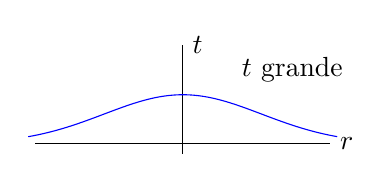
\begin{tikzpicture}[scale=1.25]

\draw (-1.5, 0) -- (1.5, 0) node[right] { $r$};
\draw (0, -0.1) -- (0, 1) node[right] {$t$};

\def\sigma{0.8};
\def\mu{0};

\draw[samples=300, domain=-pi/2:pi/2, blue] plot ({\x}, {( 1/sqrt( 2* \sigma^2 * pi)) * e^(-((\x - \mu)^ 2 ) / (2*\sigma^ 2)) });

\node[right] at (0.5, .75) {$t$ grande};

\end{tikzpicture}